
%(BEGIN_QUESTION)
% Copyright 2015, Tony R. Kuphaldt, released under the Creative Commons Attribution License (v 1.0)
% This means you may do almost anything with this work of mine, so long as you give me proper credit

Dette loopskjemaet viser et pneumatisk temperaturreguleringssystem for reaktor der en magnetventil brukes for å hjelpe aktuering av prosessventil TV-135:

$$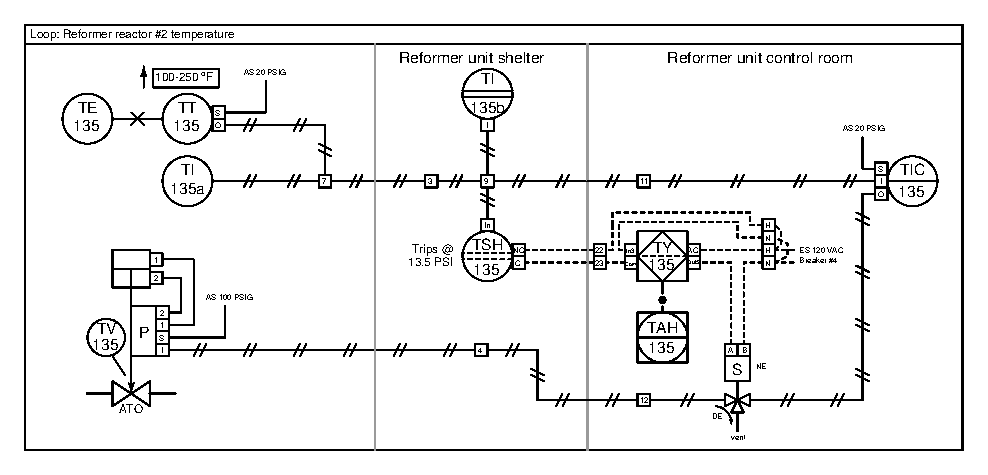
\includegraphics[width=15.5cm]{i0016rx01.eps}$$

Bestem følgende ved nøye analyse av diagrammet:

\begin{itemize}
\item{} Normal status for utgangskontakten på TY-135 ({\it NO} eller {\it NC})
\vskip 10pt
\item{} Effekt av AC-strømbrudd fra bryter \#4
\vskip 10pt
\item{} Effekt dersom ventilens avluftning tettes eller ved en feil plugges av tekniker
\end{itemize}

\underbar{file i00952}
%(END_QUESTION)





%(BEGIN_ANSWER)

\begin{itemize}
\item{} Kontaktstatus på TY-135 -- {\it TY-135 må normalt lede (lukket kontakt) for å sende AC-strøm til spolen og holde magnetventilen ``normalt energisert''.}
\vskip 10pt
\item{} Effekt av AC-strømbrudd fra bryter \#4 -- {\it spolen blir spenningsløs, lufttrykket til TV-135 ventileres ut, og ventilen går til fail-stilling (lukket).}
\vskip 10pt
\item{} Effekt av tett/plugget avluftning -- {\it hvis TY-135 kommanderer trip vil TV-135 holde posisjon i stedet for å lukke som den skal.}
\end{itemize}

%(END_ANSWER)





%(BEGIN_NOTES)


%INDEX% Documentation, loop diagram: realistic industrial example 
%INDEX% Final Control Elements, valve: fail-safe solenoids

%(END_NOTES)

